\section{Introduction}
\label{sec:intro}

\begin{figure*}[t]
  \centering
  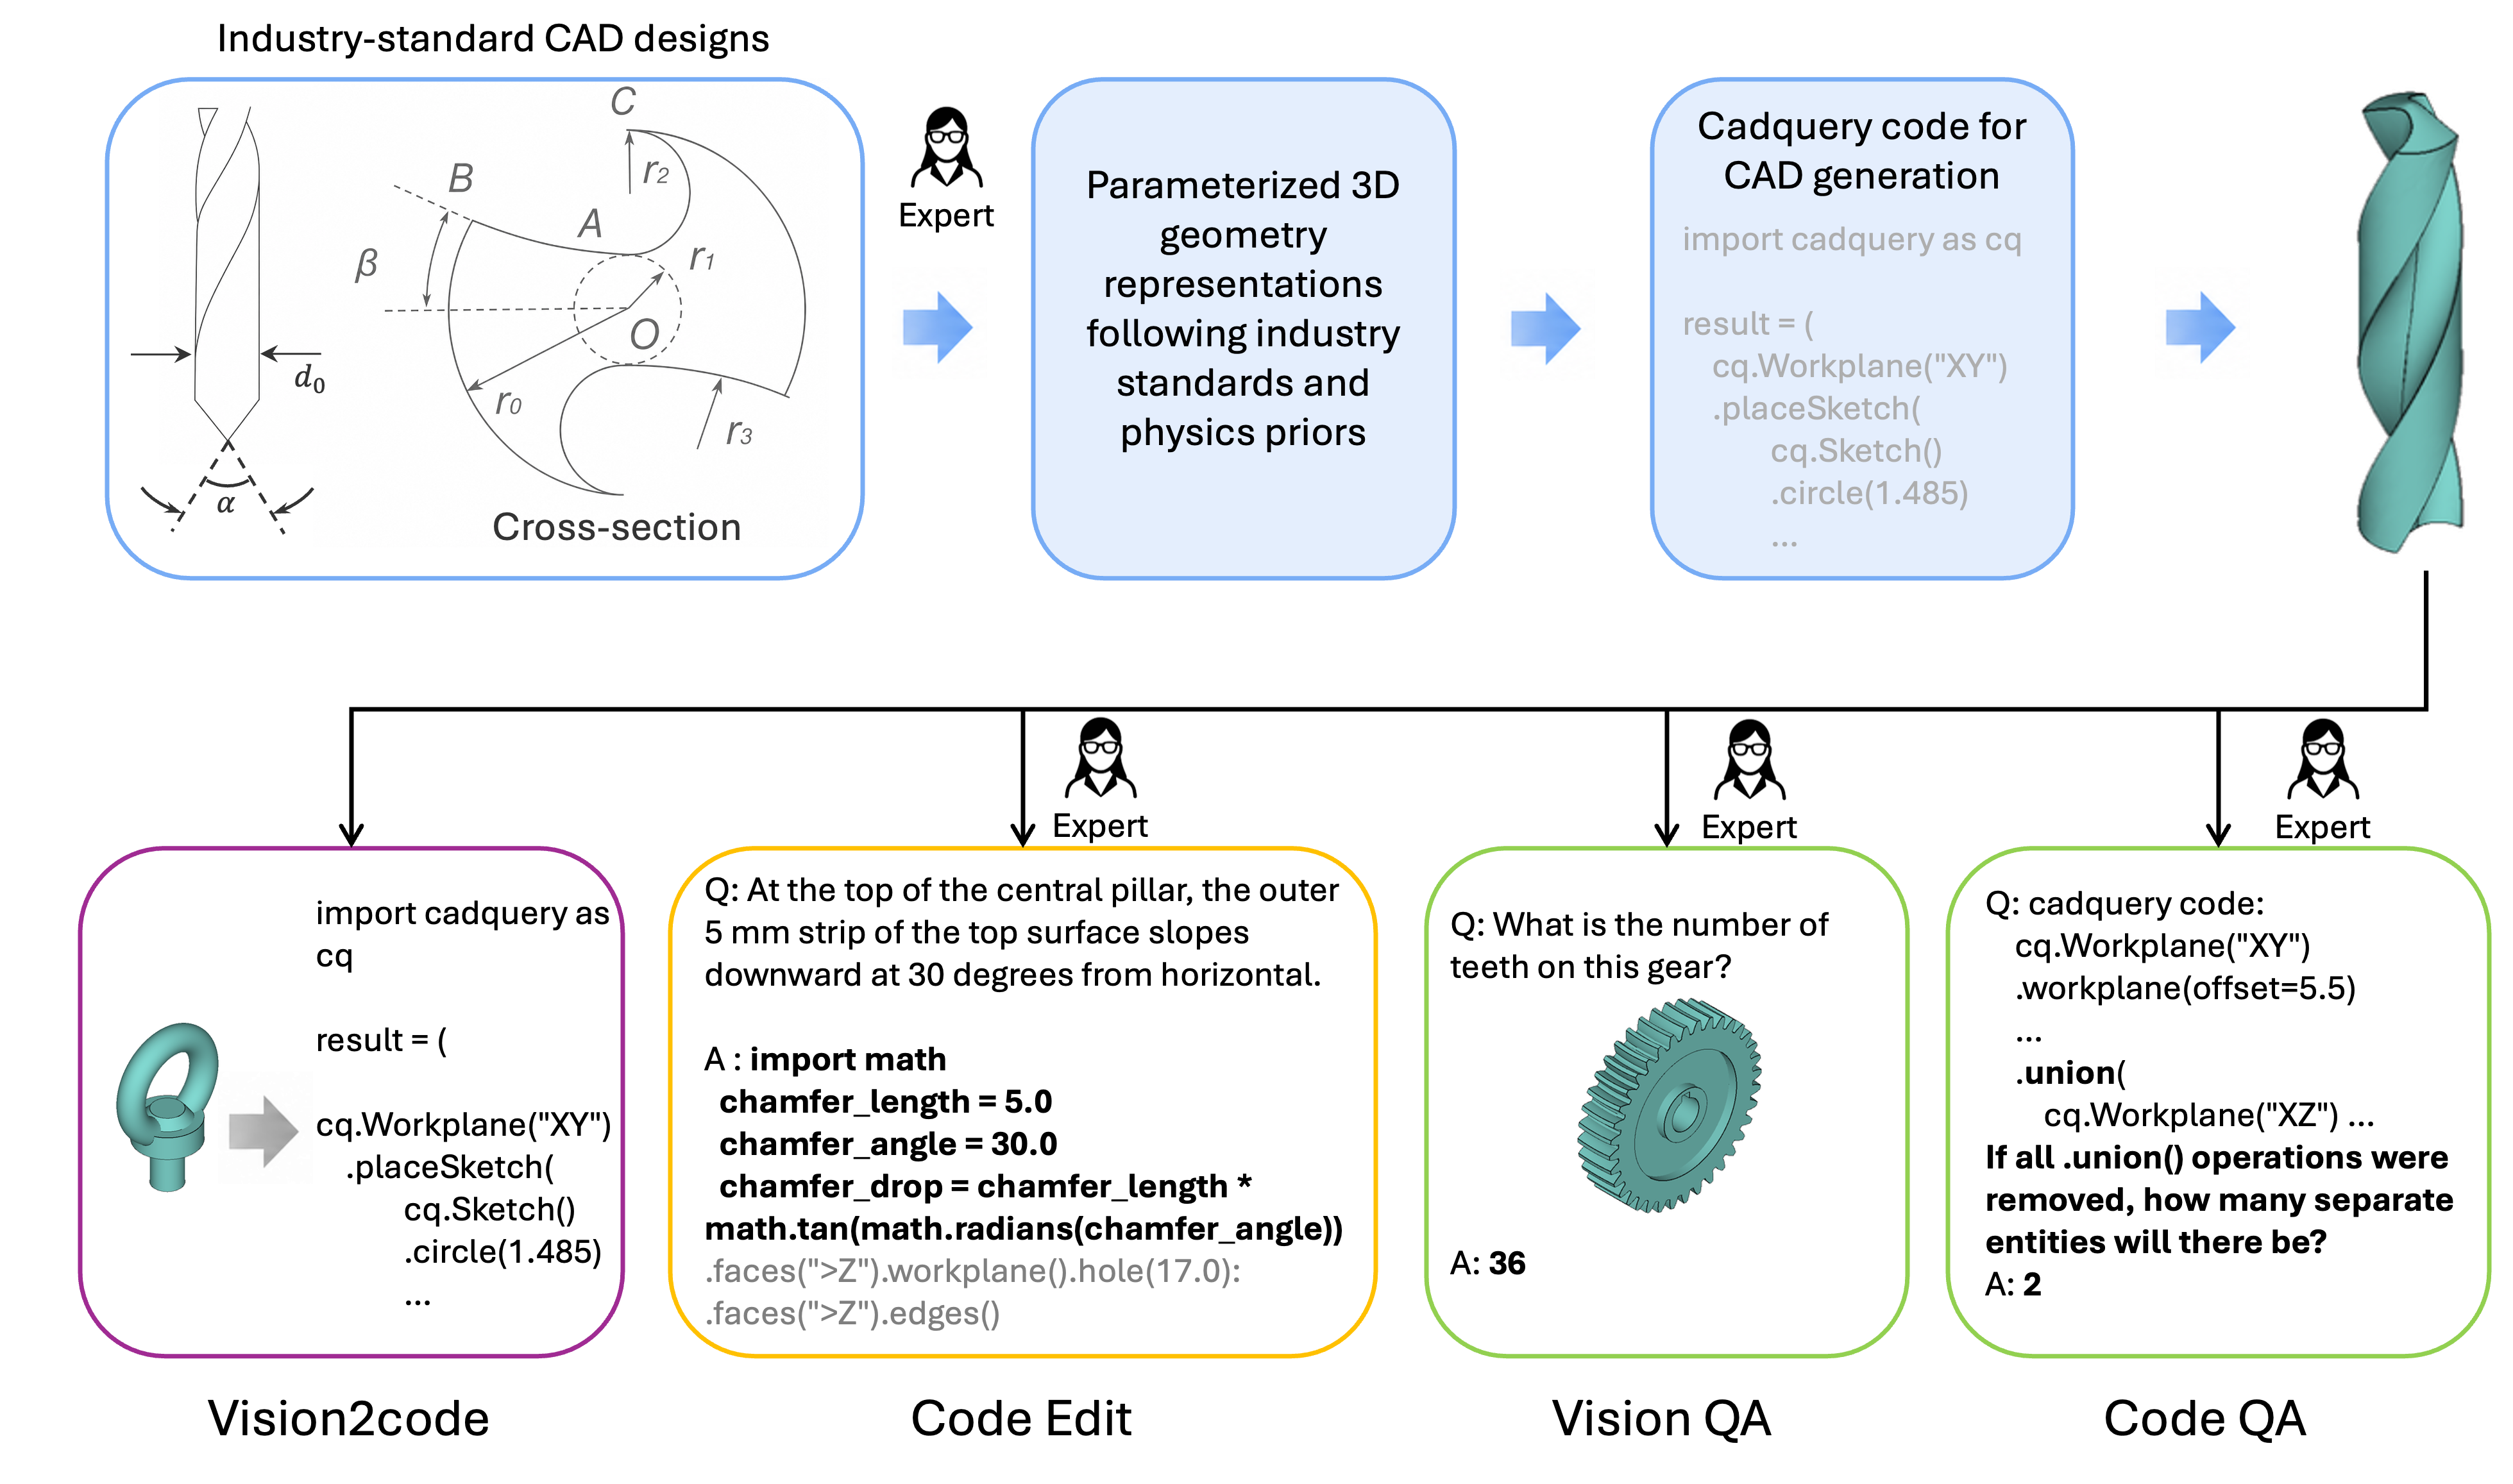
\includegraphics[width=\linewidth]{figures/fig_1.png}
  \caption{\textbf{BenchCAD overview.}
    BenchCAD evaluates multimodal models on executable and editable CAD reasoning across four tasks:
    image-to-CadQuery generation, code editing, image-based design QA, and code-based design QA.}
  \label{fig:teaser}
  \vspace{-1.8em}
\end{figure*}

Recent multimodal large language models (MLLMs) have begun to combine visual perception, code generation, and multi-step reasoning in a single interface.
This progress raises a natural question: can such models move beyond recognizing visual content to producing executable programs that define and modify physical objects?
Computer-aided design (CAD) provides a canonical setting for this question.
Unlike a mesh, point cloud, or rendered image, a CAD model is typically an editable parametric program: geometric operations such as extrusion, cutting, sweeping, filleting, and patterning construct a solid object through variables and constraints.
A capable CAD agent therefore requires more than visual recognition or code completion alone; it must connect visual evidence, 3D structure, symbolic operations, and executable program synthesis.

This makes CAD a promising application domain for MLLMs.
A useful CAD assistant should be able to read multi-view images or engineering sketches, infer the underlying 3D structure, answer design questions, generate executable CAD code, and edit existing programs while preserving unrelated geometry.
At the same time, CAD is also a challenging testbed for general AI capabilities.
Real designs are rarely arbitrary shapes.
They often belong to reusable families such as gears, springs, brackets, fasteners, pipes, and bearings, where small local details and parameter relations determine whether a part is merely visually similar or actually useful as an editable design.
For example, a spring is not fully specified by its helical silhouette; its end coils, pitch profile, and cross-section encode important design intent.
Similarly, a gear-like outline is insufficient without the correct tooth construction and parameterization.
In this sense, a model may produce geometry that passes the eye but fails the caliper.

Existing evaluations capture only parts of this problem.
3D and spatial reasoning benchmarks test whether models understand objects and viewpoints from images or code.
CAD code-generation benchmarks evaluate whether models can synthesize programs whose rendered outputs match a target shape, often using geometric metrics such as IoU or Chamfer distance.
Other datasets study program editing or design question answering in isolation.
However, these evaluations do not fully reveal whether a model has recovered the underlying parametric design logic: the part family, the construction operations, the dimensions and constraints, and the features that should remain invariant under edits.
A single end-to-end geometry score can therefore overestimate capability, because two programs may produce roughly similar outer envelopes while differing substantially in editability, operation choice, and engineering detail.

We ask: how should we evaluate whether MLLMs have the capabilities needed for practical CAD agents?
Such an evaluation should not only measure final shape similarity.
It should decompose the full CAD reasoning process into interpretable capabilities: recognizing the part and its 3D structure, understanding CAD operations, abstracting parameters and design constraints, synthesizing executable code, answering design questions, and applying localized edits without damaging non-target geometry.
This decomposition is important because failures in CAD are often compositional.
A model may identify the object family but choose the wrong operation, infer the rough scale but miss a standard relation, or edit the requested feature while unintentionally changing the rest of the part.

To address this gap, we introduce \textbf{BenchCAD}, a capability-decomposed benchmark for executable, editable, and constraint-aware CAD reasoning.
BenchCAD contains 17{,}900 execution-verified CadQuery programs across 106 industrial part families and 47 ISO/DIN/EN/ASME/IEC standards.
The dataset covers common reusable designs such as twist drills, bevel gears, compression springs, propellers, brackets, flanges, eye bolts, and fasteners.
Rather than sampling unconstrained primitive shapes, BenchCAD instantiates structured part families with meaningful parameter relations, standard-derived dimensions, and diverse CAD operations.
This allows the benchmark to test whether models can recover not only what a part looks like, but also how it should be constructed as an editable parametric program.

BenchCAD evaluates three practical CAD-agent workflows through four task families.
First, \texttt{img2cq} tests image-to-code generation: models must synthesize executable CadQuery programs from multi-view renders.
Second, \texttt{qa\_img} and \texttt{qa\_code} test design question answering from visual and program inputs, respectively, allowing us to diagnose whether failures arise from visual recognition, code understanding, operation reasoning, or parameter abstraction.
Third, \texttt{edit\_code} tests instruction-guided program editing, where the model must implement a requested local change while preserving unrelated geometry.
Together, these tasks turn CAD evaluation from a single shape-matching problem into a structured assessment of visual grounding, program synthesis, parametric reasoning, and edit preservation.

Across 10+ frontier MLLMs and open CAD-specialized baselines, BenchCAD reveals a consistent gap between apparent geometric similarity and true parametric understanding.
Current models often recognize the global part family but miss local engineering details, choose simplified or incorrect CAD operations, or fail to preserve non-target geometry during edits.
The comparison between image-based and code-based QA further shows that visual recognition alone does not imply reliable parametric abstraction.
Finally, our supervised fine-tuning (SFT) and reinforcement learning (RL) experiments show that training on BenchCAD improves operation coverage and executable generation, but substantial out-of-distribution gaps remain, especially for held-out industrial families requiring advanced operations and precise design constraints.

\paragraph{Contributions.}
Our contributions are threefold.
(i) We introduce \textbf{BenchCAD}, a domain-expert-verified dataset and generation pipeline containing 17{,}900 executable CadQuery programs across 106 industrial part families and 47 standards, together with multi-view renders, design QA pairs, and curated edit examples.
(ii) We propose a \textbf{unified CAD-agent evaluation framework} covering image-to-code generation, image/code-based QA, and instruction-guided code editing, with metrics that assess both target-task success and preservation of non-target geometry.
(iii) We provide a \textbf{capability-decomposed evaluation} of frontier MLLMs and open CAD-specialized models, showing that current systems remain limited by local detail recognition, CAD operation reasoning, parametric abstraction, and preservation-aware editing.
All data and code are anonymously released under \texttt{BenchCAD/cad\_bench} on Hugging Face under CC-BY-4.0.